\subsubsection{Multiple Features}
\begin{itemize}[--]
	\item A potential binary classification solution is to make the binary decision based on a threshold. eg. threshold = 0.5:
	\begin{align*}
		& h(x)\geq 0.5 & \text{predict } y = 1\\
		& h(x)< 0.5 & \text{predict }y = 0
	\end{align*}

	\item We want a classifier that results in $0\leq h\leq 1$, as we only have 2 outcomes 0, 1
\end{itemize}

\subsubsection{Hypothesis Representation}
\begin{itemize}[--]
	\item \textbf{Sigmoid/Logistic function}:
		$$g(z)=\frac{1}{1+e^{-z}}$$
	\begin{center}
		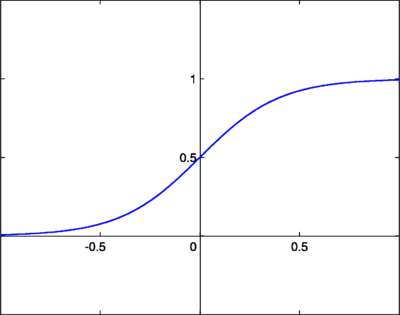
\includegraphics[scale=0.65]{sections/cs229/w3/sigmoid.png}
	\end{center}
	\item Note: there are horizontal asymptotes at 0 and 1.
	\item We will modify our original hypothesis to now be: $h(x)=g(\theta^{T}x)$, where $g$ is the previously defined sigmoid function
	\item Interpretation of hypothesis output: 
	$$h_\theta (x) = \text{ estimated probability that } y=1 \text{ on input } x$$
	\item Eg. $h(x)=0.7\to$ 70\% chance of tumor being malignant
	\item $h(x)=p(y=1|x;\theta)$ is another way of defining this.
	\item $p(y=0|x;\theta) + p(y=1|x;\theta) = 1$
\end{itemize}

\subsubsection{Decision Boundary}
\begin{itemize}[--]
	\item Suppose we predict $y=1$ if $h(x)\geq 0.5$. Graphically, we can seee that this is the same as predicting 1 when $\theta^{T}x\geq 0$
	\item \textbf{Decision Boundary}: region where $h(x)$ is equal to the threshold (the line that seperates 0 predictions vs 1 predictions).
	\item This concept can be expanded with the higher powered functions, to result in non-linear decision boundaries
	$$h(x)=g(\theta_0+\theta_1x+\theta_2 x_2 + \theta_3 x_1^2+\theta_4 x_2^2)$$
	$$\text{Predict } y=1\text{ if } -1+x_1^2+x_2^2\geq 0$$
\end{itemize}

\subsubsection{Cost Function}
\begin{itemize}[--]
	\item How do we choose/fit the parameters $\theta$?
	\item We abstract our linear regression cost function to be:
		$$j(\theta)=\frac{1}{m}\sum_{i=1}^{m}\frac{1}{2}(h(x^{(i)}-y^{(i)}))^2=\frac{1}{m}\sum_{i=1}^m\text{cost}(h(x^{(i)}, y)$$
		$$\text{cost}(h(x), y)=\frac{1}{2} (h(x)-y)^2$$

	\item However, this cost function is non-convex for logistic regression, which doesn't allow us to run gradient descent (no garuntee of global minimum reached).
	\item Let our cost function for logistic regression now be defined as:
	$$\text{cost}(h(x), y)=\begin{cases}
		-\log (h(x)) & y=1 \\
		-\log (1-h(x)) & y=0
	\end{cases}$$
	\begin{center}
		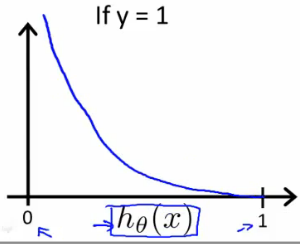
\includegraphics[scale=0.7,]{sections/cs229/w3/logisticcost.png}
		\newline
		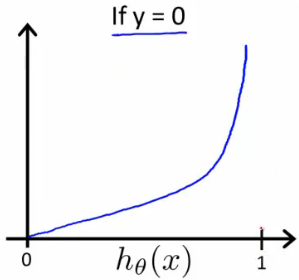
\includegraphics[scale=0.]{sections/cs229/w3/logisticcost0.png}
	\end{center}

	\item This allows us to have no cost when we were correct at our guess, but have increasingly greater cost the more wrong we were.
\end{itemize}

\subsubsection{Simplified Cost Function and Gradient Descent}
\begin{itemize}[--]
	\item j
\end{itemize}